\chapter{Implementation}
In this chapter I will describe the implementation of the language and the plugin, the problems faced and the solutions adopted.

\section{The plugin}
For the implementation of the Burp's plugin introduced earlier, I have decided to start from a work done by my colleague Wendy Barreto \cite{wendy_barreto} in her bachelor thesis, which realized a similar plugin for OIDC and OAuth SSO protocols, this was a good base to start with my implementation. The interface of \cite{wendy_barreto} has been taken and adapted to fit the needs of this work. The plugin code is written in Java, I used the Burp's interface classes to interact with it.
The standard usage of Burp Suite is based on the execution of a browser which connects to the Burp's proxy, in a way that all the packets can be intercepted, viewed or edited and forwarded or dropped from the Burp interface. The tester would do some actions on the browser and watch the flowing packets in Burp and then check them or edit them. With the plugin the idea is the same, but the operation done on the browser and the checks or edits on the messages are made automatically, in a way that the tester doesn't have to do them by itself.

\subsection{The interface}
In figure \ref{fig:plugin_interface} we can see the interface of the plugin, starting from top left we have the session track input space, where it can be specified a different track for each session. Following on the top right, wee have a series of buttons that allow various configurations:
\begin{itemize}
    \item the browser to be used can be selected
    \item the driver to automate the actions on the browser can be selected
    \item the record button can be used to record the passing messages
    \item the load messages button can be used to load the previously saved messages to be tested "offline"
    \item the offline mode button to test the loaded messages instead of the live ones
\end{itemize}

In the bottom we have multiple tabs:
\begin{itemize}
    \item "Input JSON" tab is used to load the tests written in the language into the plugin, and with the use of two buttons we can parse the language and execute the tests.
    \item "Test suite result" is the tab containing all the results of the executed tests
    \item "Test result" is the tab used to see the specific test result, with all the intercepted messages related to it
    \item "Session config" is used to configure the ports of the sessions that will be used in the tests.
\end{itemize}

\begin{figure}
    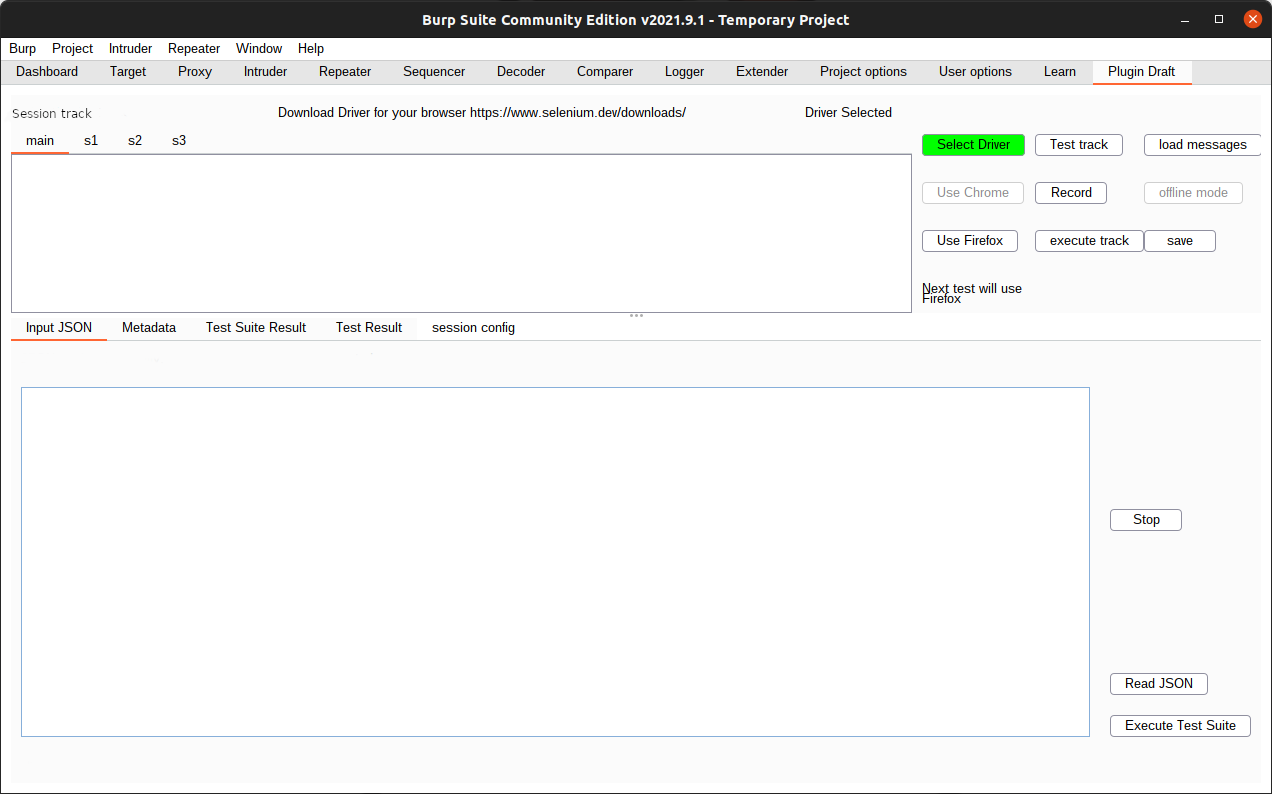
\includegraphics[width=\textwidth]{interface.png}
    \caption{plugin interface}
    \label{fig:plugin_interface}
\end{figure}

\subsection{Test execution}
The test execution differs from static to dinamic, as static tests don't need the the edit of the messages, the execution of the \gls{session track} is done once, the messages are saved and the tests are executed on the saved messages. I have also added the possibility of exporting the saved messages to a file, in a way that they can be imported in the plugin and tested again.
On the other hand, active tests needs to edit the messages, so the execution of the track has to be repeated for each test.

\subsection{Decoding \& encoding of parameters}
As said in the previous chapter, the encoding and decoding of parameters is possible. To do that, a list of encodings has to be provided, i.e. url, base64, deflate. Once the specified message is intercepted, the parameter is taken and decoded following the order of the provided encodings. To do that, i used part of the code of SAML Raider \cite{saml_raider} which did the decoding of SAML Requests and responses parameters. I've taken that part of the code and edited it to fit the plugin. SAML Raider is a Burp's plugin used to manage SAML certificates.

\subsection{SAML certificate managing}
In SAML Requests and responses there is sometime the need to remove or edit the certificate associated to that request or response, so, to speed up the process I did add a specific tag in the language to remove or edit the certificate signature. There is still the possibility of doing it by editing the SAML request or response with a regex, but this way is more convinient.
To do this, i used a part of the code of SAML Raider \cite{saml_raider}, editing it to fit my needs.

\subsection{Oracle}

To identify abnormal pages like error pages the \gls{session track} evaluation should be sufficient, because if some of the actions could not be executed means that the original "flow" of pages was not followed.

\subsection{Session managing}
The sessions are managed independently, each session is basically a browser that is launched when a session is started. Each session can follow a different \gls{session track} defined in the apposite tabs. Every session is ran in a separated thread to make parallelism possible. By the use of specific commands in the language, is possible to do some actions on each session, like stop it, pause it, or clear its cookies. Each browser uses a different proxy port, so that it is possible to know from which session the messages come from.




